\newif\ifglobal

%%%%%%%%%%%%%%%%%%%%%%%
%%% Compile to view %%%
%%%%%%%%%%%%%%%%%%%%%%%

%%%%%%%%%%%%%%%%%%%%%%%%%%%%%%%%%%%%%%%%%%%%%%%%%%%
%%% Readme:                                     %%%
%%% https://www.overleaf.com/read/bwdjvfjksvjy/ %%%
%%%%%%%%%%%%%%%%%%%%%%%%%%%%%%%%%%%%%%%%%%%%%%%%%%%

% >>> M?: marks a module setting number or important notice

% >>> M4: Set {./relative-path} to external files for this module <<<
\def \modulefiles {./11-DIGSIG}
% To add an external file, use:
% (Replace '---' with actual filename)
% '\input{\modulefiles/tables/---.tex}' for tables
% '\includegraphics{\modulefiles/figures/---}' for figures
% '\subfile{\modulefiles/---}' for register files


% >>> M1: This module is in global project? <<<
% 'YES' - uncomment; 'NO' - comment out
\globaltrue

\ifglobal
    \documentclass[main\_\_CN.tex]{subfiles}
   
\else
    % Font "FandolSong-Regular" used by ctex does not have GSUB table.
    % It causes warnings that do not affect compilation and can be ignored.
    \PassOptionsToPackage{quiet}{fontspec}

    \documentclass[openany, 10pt]{book}
   
    % >>> M2: In ./00-shared/preamble-trm-module, also find
    %         settings for visibility of todo notes, watermark <<< 
    \usepackage{preamble-trm-module}


    % Enable Chinese typesetting
    \usepackage{ctex}

    % >>> M3: Temporary labels in Chinese
    %         you can add your own labels there <<<
    \myexternaldocument{./00-shared/temp-labels-cn}

\fi %\ifglobal


\setcounter{secnumdepth}{4}


% >>> M5: If this module needs any updates in
% './00-shared/preamble-trm-module.sty'
% (include additional package, etc.), contact your module PM
% or create the file './00-shared/changelog.tex' make the
% necessary updates yourself and document them in this file <<<


\begin{document}


% Sets language into which pre-defined bits of text are translated
\selectlanguage{chinese}

% Do not delete this block
\ifglobal
% Add the following front matter if
% this module is outside of global project
\else
    \InputIfFileExists{readme}{}{}
    {\let\clearpage\relax \listoftodos}
    \tableofcontents
    %\listoftables
    %\listoffigures
\fi



%%%%%%%%%%%%%%%%%%%%%%%%%
%%% TRM Module Begins %%%
%%%%%%%%%%%%%%%%%%%%%%%%%

\chapter{RSA 数字签名外设 (RSA\_DS)}
\label{mod:digsig}
\hypertarget{digsig}{}\hypertarget{rsads}{}


\section{概述}

数字签名技术在密码学算法层面上用于验证消息的真实性和完整性。这可用于向服务器验证设备自身身份，或验证消息是否未被篡改。

\chipname{} 包含一个 RSA 数字签名外设 (RSA\_DS)，可基于 RSA 高效生成数字签名。RSA\_DS 外设使用预先加密的参数计算出签名，HMAC 作为密钥导出函数加密这些参数。反过来， HMAC 则使用 eFuse 作为输入密钥。上述整个过程都发生在硬件层面，因此在计算过程中，不论是解密 RSA 参数的密钥还是用于 HMAC 密钥导出函数的输入密钥都对用户不可见。

\section{主要特性}

\begin{itemize}
\item RSA 数字签名支持密钥长度最大为 3072 位
\item 私钥数据已加密，并且只能由 RSA\_DS 外设读取
\item SHA-256 摘要用于保护私钥数据免遭攻击者篡改
\end{itemize}


\section{功能描述}
\subsection{概述}

RSA\_DS 外设计算 RSA 签名操作 \begin{math}Z = X^{Y} \bmod M\end{math}，其中 \begin{math}Z\end{math} 是签名，\begin{math}X\end{math} 是输入消息，\begin{math}Y\end{math} 和 \begin{math}M\end{math} 是 RSA 私钥参数。

私钥参数以密文形式存储在 flash 中。对其解密而使用的密钥（\begin{math} RSA\_DS\_KEY \end{math}） 只能由 RSA\_DS 外设通过 HMAC 模块获取，并且 HMAC 模块求解该密钥所需的一切输入信息（\begin{math} HMAC\_KEY \end{math}）只存放在 eFuse 中且只允许被 HMAC 模块访问。这意味着只有 RSA\_DS 硬件才能解密私钥密文，软件获取不到私钥明文。关于 eFuse 和 HMAC 的相关细节请参照章节 \ref{mod:efuse} \textit{\nameref{mod:efuse}} 和 章节 \ref{mod:hmac} \textit{\nameref{mod:hmac}}。

需要签名时，软件直接将输入消息 \begin{math}X\end{math} 发送到 RSA\_DS 外设。RSA 签名计算完成后，软件将读取签名结果 \begin{math}Z\end{math}。


为方便描述，这里约定几个符号，它们的作用域局限于本章。

\begin{itemize}
\item 
1\begin{math}^s\end{math} 
\hspace{0.75cm} 
表示一个完全由 “1” 组成的长度为 \begin{math}s\end{math} 位的位串。

\item
    \begin{math}[x]_{s}\end{math}  \hspace{0.5cm}
       一个长度为 \begin{math}s\end{math} 位的位串，要求 \begin{math}s\end{math} 为 8 的整数倍。如果 \begin{math}x\end{math} 是一个数 (\begin{math}x\end{math} < 2\begin{math}^s\end{math})， 那么其在位串中遵循小端字节序。\begin{math}x\end{math} 可以是一个变量，例如 \begin{math}[Y]_{4096}\end{math}，或一个十六进制的常数，比如 [0x0C]\begin{math}_{8}\end{math}。根据需要，\begin{math}[x]_{t}\end{math} 右边可以加上\begin{math} (s-t) \end{math} 个 0，使字串长度扩展成 \begin{math}s\end{math} 位，得到 \begin{math}[x]_{s}\end{math}。例如：
       [0x05]\begin{math}_{8} = 00000101\end{math}，
       [0x05]\begin{math}_{16} = 00000101 00000000\end{math}，
       [0x0005]\begin{math}_{16} = 00000000 00000101\end{math}，
       [0x13]\begin{math}_{8} = 00010011\end{math}，
       [0x13]\begin{math}_{16} = 00010011 00000000\end{math}，
       [0x0013]\begin{math}_{16} = 00000000 00010011\end{math}。

    \item 
        \begin{math}{ || }\end{math}  \hspace{1.0cm}        表示位串粘接操作符，用于将两个位串前后粘成一个较长的位串。
\end{itemize}



\subsection{私钥运算子}
\label{sec:digsig-private-key-operands}

私钥运算子 \begin{math}Y\end{math}（私钥指数）和 \begin{math}M\end{math}（密钥模数）由用户生成。它们具有特定的 RSA 密钥长度（最大为 3072 位）。
RSA 签名操作还额外需要两个运算子，即参数 \begin{math}\overline{r}\end{math} 和 \begin{math}M^{\prime}\end{math}，这两个参数需要软件由 \begin{math}Y\end{math} 和 \begin{math}M\end{math} 运算得到。

    
运算子 \begin{math}Y\end{math}、
\begin{math}M\end{math}、
\begin{math}\overline{r}\end{math} 和
\begin{math}M^{\prime}\end{math} 与验证摘要一起由用户加密并以密文 \begin{math}C\end{math} 的形式存储。密文 \begin{math}C\end{math} 输入到 RSA\_DS 外设之后先由硬件解密，然后参与 RSA 签名运算。如何生成 \begin{math}C\end{math} 请参考章节 \ref{sec:digsig-private-key-operands}。

RSA\_DS 外设支持运算子长度为 \begin{math}N = 32 \times x\end{math} (\begin{math}x \in \{ 1,2,3, \dots, 96\} \end{math}) 的 RSA 签名运算 \begin{math}Z = X^{Y} \bmod M\end{math}，需要满足 RSA 计算的运算子长度要求，即 \begin{math}Z\end{math}、
\begin{math}X\end{math}、
\begin{math}Y\end{math}、
\begin{math}M\end{math} 和 
\begin{math}\overline{r}\end{math}
的位宽必须相同，但必须为这 96 种中的其中一种，
而 \begin{math}M^{\prime}\end{math} 的位宽始终是 32。
更多 RSA 计算相关信息请参考章节 \ref{mod:rsa} \textit{\nameref{mod:rsa}} 中的 \ref{sec:rsa-large-modular-Exponentiation} \textit{\nameref{sec:rsa-large-modular-Exponentiation}} 部分。


\subsection{软件需要做的准备工作} 
\label{sec:digsig-prerequisities}

如果用户想使用 RSA\_DS 外设进行数字签名，软件和硬件必须紧密配合才可以顺利完成，并且软件需要做一系列准备工作，如图 \ref{fig:digsig-flow} 所示。图中左半边给出了在硬件开始 RSA 签名计算之前，软件需要做哪些准备工作。图中右半边展示了硬件在整个签名计算的过程中具体会做些什么。

\begin{figure}[H]
    \centering
    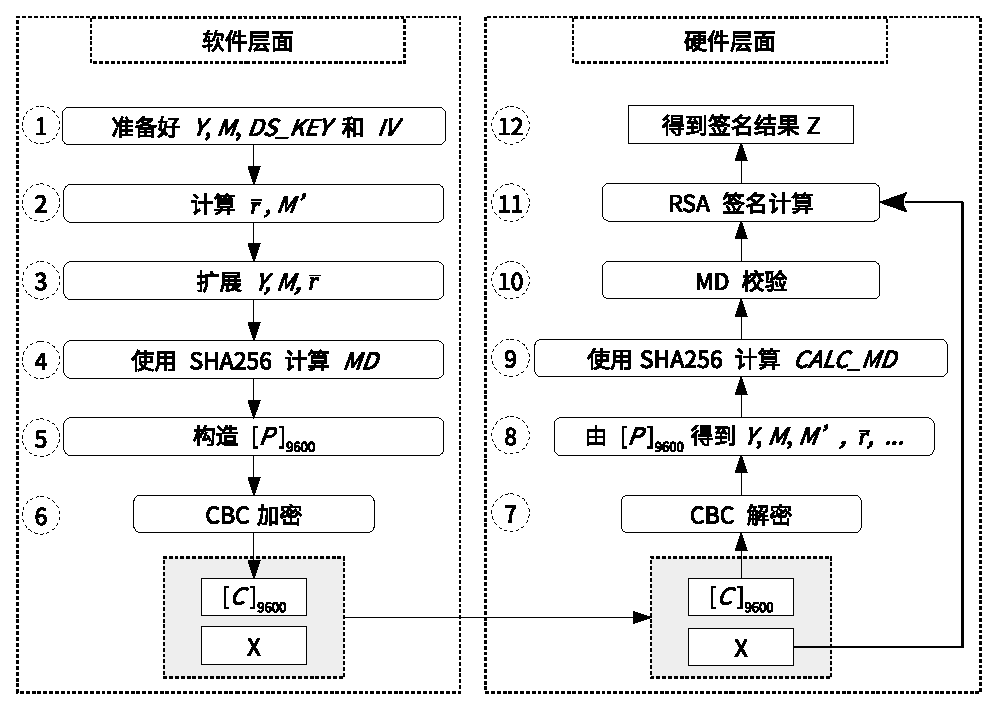
\includegraphics[width=0.7\textwidth]{./11-DIGSIG/figures/11-DIGSIG-flow__CN}
    \caption{软件准备工作与硬件工作流程}
    \label{fig:digsig-flow}
\end{figure}


\begin{tiplisting}
\vspace{-2.5em}
\begin{enumerate}
\item 对于多次签名计算，软件准备工作（图 \ref{fig:digsig-flow} 左侧）只需要进行一次，但对于每一次签名计算，硬件运算（图 \ref{fig:digsig-flow} 右侧）都需要重新进行。
\end{enumerate}
\end{tiplisting}


用户需要依照图 \ref{fig:digsig-flow} 指定的步骤来计算 \begin{math}C\end{math}。详细的过程描述如下：

\begin{itemize}

    \item {\bfseries 步骤 1}：按照章节 \ref{sec:digsig-private-key-operands} 所述准备好 RSA 私钥运算子 \begin{math}Y\end{math} 和 \begin{math}M\end{math}，它们应符合运算子的长度要求。
          记 \begin{math}[L]_{32} = \frac{N}{32}-1 \end{math}（比如，对于 RSA 3072，\begin{math}[L]_{32}\end{math} == [0x60-1]\begin{math}_{32}\end{math}）。还需要准备好 \begin{math}[HMAC\_KEY]_{256}\end{math}，并计算出 \begin{math}[DS\_KEY]_{256}\end{math}， 即 \begin{math}DS\_KEY\end{math} = HMAC-SHA256(\begin{math}[HMAC\_KEY]_{256}\end{math}, \begin{math}1^{256}\end{math})。 另外还需要引入一个随机的 \begin{math}[IV]_{128}\end{math}， 它需要符合 AES-CBC 块加密算法的要求。有关 AES 更多信息，请参考章节 \ref{mod:aes} \textit{\nameref{mod:aes}}。 
    
    \item {\bfseries 步骤 2}：
          根据 \begin{math}M\end{math} 求解 \begin{math}\overline{r}\end{math} 和 \begin{math}M^{\prime} \end{math}。
    
    \item {\bfseries 步骤 3}：
          扩展 \begin{math}Y\end{math}、
               \begin{math}M\end{math} 和 
               \begin{math}\overline{r}\end{math}，
          得到 \begin{math}[Y]_{3072}\end{math}、
               \begin{math}[M]_{3072}\end{math} 和
               \begin{math}[\overline{r}]_{3072}\end{math}。
          由于 \begin{math}Y\end{math}、\begin{math}M\end{math} 和 \begin{math}\overline{r}\end{math} 的最大位宽为 3072，运算子位宽小于 3072 的运算子 需要扩展至 3072，位宽等于 3072 则不需要扩展。
       
    
    \item {\bfseries 步骤 4}：
            使用 SHA-256 计算 MD 校验码： 
                \begin{math}[MD]_{256}\end{math} = SHA256 (\begin{math} 
                [Y]_{3072} ||
                [M]_{3072} ||
                [\overline{r}]_{3072} ||
                [M^{\prime}]_{32} ||
                [L]_{32} ||
                [IV]_{128} 
            \end{math})

    \item {\bfseries 步骤 5}：构造 \begin{math}[P]_{9600}\end{math} = (
            \begin{math}
                [Y]_{3072} ||
                [M]_{3072} ||
                [\overline{r}]_{3072} ||
                [Box]_{384}
            \end{math}) 。
            这里 \begin{math}[Box]_{384}\end{math} = (
            \begin{math}
                [MD]_{256} ||
                [M^{\prime}]_{32} ||
                [L]_{32} ||
                [\beta]_{64}) 
            \end{math}，
            其中 \begin{math}[\beta]_{64} \end{math} 是符合 PKCS\#7 封装方式的追加码， 由 8 个 字节码 0x80 组成，即 $[$0x0808080808080808$]_{64}$，目的在于使 \begin{math}P\end{math} 的长度为 128 位的整数倍。
    
    \item {\bfseries 步骤 6}：
            计算密文形式的私钥参数 \begin{math}C\end{math} = \begin{math}[C]_{9600}\end{math} = 
            AES-CBC-ENC (\begin{math}[P]_{9600}\end{math}, \begin{math}[DS\_KEY]_{256}\end{math}, \begin{math}[IV]_{128}\end{math})，长度为 1200 字节。
            \begin{math}C\end{math} 也可以表示为
            \begin{math}C\end{math} = \begin{math}[C]_{9600}\end{math} = 
            (\begin{math}
            [\widehat{Y}]_{3072} ||
            [\widehat{M}]_{3072} ||
            [\widehat{ \overline{r} }]_{3072} ||
            [\widehat{Box}]_{384} 
            \end{math})，
            其中
            \begin{math} [\widehat{Y}]_{3072} \end{math}、
            \begin{math} [\widehat{M}]_{3072} \end{math}、
            \begin{math} [\widehat{ \overline{r} }]_{3072} \end{math}、
            \begin{math} [\widehat{Box}]_{384} \end{math}
            是 \begin{math}C\end{math} 的四个子参数，分别对应
            \begin{math} [Y]_{3072} \end{math}、
            \begin{math} [M]_{3072} \end{math}、
            \begin{math} [\overline{r}]_{3072} \end{math}、
            \begin{math} [Box]_{384} \end{math}
            的密文形式。
    
\end{itemize}

\subsection{硬件工作流程}
\label{sec:digsig-hardware-level-operation}

每次需要计算数字签名时，都会触发硬件操作。硬件需要三个输入信息：预先生成的私钥密文 \begin{math}C\end{math}、唯一的消息 \begin{math}X\end{math}、 \begin{math}IV\end{math}。

RSA\_DS 外设的工作流程可以分为如下三个阶段：

\begin{enumerate}  

    \item {\bfseries 解析阶段，即图 \ref{fig:digsig-flow} 中的步骤 7 和 步骤 8}
    
        解析过程是图 \ref{fig:digsig-flow} 中步骤 6 的逆过程。RSA\_DS 外设将调用 AES 硬件加速器以 CBC 块模式对输入的密文信息 \begin{math}C\end{math} 进行解密，获取明文信息。
        该过程可以表示为
        \begin{math}P\end{math} = AES-CBC-DEC (\begin{math}C\end{math}, \begin{math}DS\_KEY\end{math}, \begin{math}IV\end{math})，其中 \begin{math}IV\end{math} 就是 \begin{math}[IV]_{128}\end{math}，由用户直接指定； \begin{math}[DS\_KEY]_{256}\end{math} 由硬件 HMAC 提供，由 存储在 eFuse 中的 \begin{math}HMAC\_KEY\end{math} 得到，软件无法获取。请参考章节 \ref{mod:hmac} \textit{\nameref{mod:hmac}} 获取更多信息。
        
        显然，RSA\_DS 外设能够通过 \begin{math}P\end{math} 解析出 \begin{math}[Y]_{3072}\end{math}、\begin{math}[M]_{3072}\end{math}、\begin{math}[\overline{r}]_{3072}\end{math}、\begin{math}[M^{\prime}]_{32}\end{math}、\begin{math}[L]_{32}\end{math}、MD 校验码和追加码 \begin{math}[\beta]_{64} \end{math}，这相当于步骤 5 的逆过程。
        
    \item {\bfseries 校验阶段，即图 \ref{fig:digsig-flow} 中的步骤9 和 步骤 10}
        
        RSA\_DS 外设会执行两种校验操作： MD 校验和填充 (padding) 校验。 
        由于填充校验和 MD 校验同步进行， 因此填充校验不在图 \ref{fig:digsig-flow} 中体现。 
        
        
        \begin{itemize}
    
            \item MD 校验 —— RSA\_DS 外设调用 SHA-256 进行哈希计算获取哈希值 \begin{math}[CALC\_MD]_{256}\end{math}（即步骤 4），然后将 \begin{math}[CALC\_MD]_{256}\end{math} 与 MD 校验码 \begin{math}[MD]_{256}\end{math} 作比较，当且仅当二者相同时，MD 校验通过。
            
            \item 填充校验 —— RSA\_DS 外设将检查解析阶段解析出的 追加码 \begin{math}[\beta]_{64} \end{math} 是否符合 PKCS\#7 标准，当且仅当符合标准时，填充校验通过。
                    
        \end{itemize}
        
        如果 MD 校验通过，RSA\_DS 外设将执行后续计算；否则 RSA\_DS 外设拒绝执行。
        如果填充校验失败，将生成警告信息，但不会影响 RSA\_DS 外设的后续操作。
    
    \item {\bfseries 计算阶段，即图 \ref{fig:digsig-flow} 中的步骤 11 和步骤 12}
    
        RSA\_DS 外设将把用户输入的 \begin{math}X\end{math}，
        以及解析得到的 \begin{math}Y\end{math}、\begin{math}M\end{math} 和 \begin{math}\overline{r}\end{math} 都视为大数，结合解析得到的 \begin{math}M^{\prime}\end{math}，构成了大数模幂运算 \begin{math} X^{Y} \bmod M\end{math} 的所有必要输入参数。大数模幂运算的运算长度由 \begin{math}L\end{math} 的值唯一指定。RSA\_DS 外设调用 RSA 硬件加速器完成大数模幂运算 \begin{math}Z = X^{Y} \bmod M\end{math}，\begin{math}Z\end{math} 为签名结果。

\end{enumerate}


\subsection{软件工作流程}

每次需要计算数字签名时，都应执行以下软件操作。输入消息是预先生成的私钥密文 \begin{math}C\end{math}、唯一的消息 \begin{math}X\end{math}、 \begin{math}IV\end{math}。这些软件步骤触发章节 \ref{sec:digsig-hardware-level-operation} 中描述的硬件工作流程。下述流程基于一个假设：软件已经调用了 HMAC 外设，硬件上 HMAC 已经根据 \begin{math}HMAC\_KEY\end{math} 计算出了 \begin{math}RSA\_DS\_KEY\end{math}。

\begin{enumerate}
    
    \item {\bfseries 准备工作}：准备好 \begin{math}C\end{math}、\begin{math}X\end{math}、 \begin{math}IV\end{math}。具体方法请参考章节 \ref{sec:digsig-prerequisities} 。
    
    \item {\bfseries 启动 RSA\_DS 外设}：对寄存器 \hyperref[regdesc:DSSETSTARTREG]{DS\_SET\_START\_REG} 写 1。
    
    \item {\bfseries 检查 \begin{math}RSA\_DS\_KEY\end{math} 是否已经准备好}：轮询寄存器 \hyperref[regdesc:DSQUERYBUSYREG]{DS\_QUERY\_BUSY\_REG} 直到读到 0。
    
    如果 \hyperref[regdesc:DSQUERYBUSYREG]{DS\_QUERY\_BUSY\_REG} 超过 1 ms 还没读到 0，则说明 HMAC 未被调用。此时，软件应当读寄存器 \hyperref[regdesc:DSQUERYKEYWRONGREG]{DS\_QUERY\_KEY\_WRONG\_REG}，根据返回值判断具体是哪一种情况。 
    \begin{itemize}
    
        \item 如果读到零值，说明 HMAC 未被调用。
        
        \item 如果读到非零值 (1 \verb+~+ 15)，则说明 HMAC 被调用过，但是 RSA\_DS 外设没有拿到 \begin{math}RSA\_DS\_KEY\end{math}，原因可能是有其他程序的干扰。
        
    \end{itemize}
    
    \item {\bfseries 配置寄存器}：将 \begin{math}IV\end{math} block 写入寄存器 DS\_IV\_\textcolor{red}{\it{m}}\_REG (\textcolor{red}{\it{m}}: 0 \verb+~+ 3)。有关 \begin{math}IV\end{math} block 的更多信息，请参考章节 \ref{mod:aes} \textit{\nameref{mod:aes}}。

    \item {\bfseries 将 \begin{math}X\end{math} 写入存储器 \hyperref[DSXMEM]{DS\_X\_MEM}}：将 \begin{math}X_{i}\end{math}
        (\begin{math}i \in \{ 0, 1, \dots, n-1 \end{math} \} )
        写入存储器 \hyperref[DSXMEM]{DS\_X\_MEM}，容量为 96 个字 (word)，其中 \begin{math} n = \frac{N}{32} \end{math} 。
        每一个字刚好存放一个 \begin{math}b\end{math} 进制数。存储器的低地址存放运算子的低位进制数，高地址存放运算子的高位进制数。当 \begin{math}X\end{math} 的长度小于 96 个字时，存储器 \hyperref[DSXMEM]{DS\_X\_MEM} 中有一部分空间未使用，该部分空间中的数据可以是任意值。
        
    \item {\bfseries 将 \begin{math}C\end{math} 写入存储器}：即将 \begin{math}C\end{math} 中的四个子参数分别写入对应的存储器。
    \begin{itemize}
        
        \item 将 \begin{math}\widehat{Y}_{i}\end{math}
        (\begin{math}i \in \{ 0, 1, \dots, 95 \} \end{math})
        写入存储器 \hyperref[DSYMEM]{DS\_Y\_MEM}。
        
        \item 将 \begin{math}\widehat{M}_{i}\end{math}
        (\begin{math}i \in \{ 0, 1, \dots, 95 \} \end{math})
        写入存储器 \hyperref[DSMMEM]{DS\_M\_MEM}。
        
        \item 将 \begin{math}\widehat{\overline{r}}_{i}\end{math}
        (\begin{math}i \in \{ 0, 1, \dots, 95 \} \end{math})
        写入存储器 \hyperref[DSRBMEM]{DS\_RB\_MEM}。
        
        \item 将 \begin{math}\widehat{Box}_{i}\end{math}
        (\begin{math}i \in \{ 0, 1, \dots, 11 \} \end{math})
        写入存储器 \hyperref[DSBOXMEM]{DS\_BOX\_MEM}。
        
        其中 存储器 
        \hyperref[DSYMEM]{DS\_Y\_MEM}、
        \hyperref[DSMMEM]{DS\_M\_MEM}、
        \hyperref[DSRBMEM]{DS\_RB\_MEM} 的
        容量均为 96 个字，
        而存储器 \hyperref[DSBOXMEM]{DS\_BOX\_MEM} 容量只有 12 个字。
        每一个字刚好存放一个 \begin{math}b\end{math} 进制数。
        存储器的低地址存放运算子的低位进制数，高地址存放运算子的高位进制数。
    
    \end{itemize}

    \item {\bfseries 启动计算}：对寄存器 \hyperref[regdesc:DSSETMEREG]{DS\_SET\_ME\_REG} 写入 1。

    \item {\bfseries 等待运算结束}：轮询寄存器 \hyperref[regdesc:DSQUERYBUSYREG]{DS\_QUERY\_BUSY\_REG} 直到读到 0。

    \item {\bfseries 检查校验结果}：读寄存器 \hyperref[regdesc:DSQUERYCHECKREG]{DS\_QUERY\_CHECK\_REG}，根据返回值决定后续操作。
    
    \begin{itemize}
    
        \item 如果返回值为 0，则说明填充校验通过，MD 校验通过，可以继续读取 \begin{math}Z\end{math} 结果值。
        
        \item 如果返回值为 1，则说明填充校验通过，但 MD 校验失败。\begin{math}Z\end{math} 结果值全零无效，跳至步骤 \ref{other:digsig-step-exit}。
        
        \item 如果返回值为 2，则说明填充校验通过失败，但 MD 校验通过，用户可以继续读取 \begin{math}Z\end{math} 结果值。但仍需注意的是，数据填充不符合 PKCS\#7 封装方式，这可能不是你想要的。
        
        \item 如果返回值为 3，则说明填充填充校验失败，且 MD 校验失败。 这种情况说明有致命错误发生。\begin{math}Z\end{math} 结果值全零无效。跳至步骤 \ref{other:digsig-step-exit}。
        
    \end{itemize}
        
    \item {\bfseries 读出运算结果}：从存储器 \hyperref[DSZMEM]{DS\_Z\_MEM} 读出运算结果 \begin{math}Z_{i}\end{math} (\begin{math}i \in \{0,1, \dots,n-1\}\end{math})，其中 \begin{math} n = \frac{N}{32} \end{math} 。\begin{math}Z\end{math} 以小端字节序存储在存储器中。
    
    \item {\bfseries 退出计算环境\label{other:digsig-step-exit}}：对寄存器 \hyperref[regdesc:DSSETFINISHREG]{DS\_SET\_FINISH\_REG} 写入 1，然后轮询寄存器 \hyperref[regdesc:DSQUERYBUSYREG]{DS\_QUERY\_BUSY\_REG} 直到读到 0。

\end{enumerate}

RSA\_DS 外设退出计算环境后，所有输入/输出寄存器和存储器中的数据都已经被抹除（清零）。

\clearpage
\section{ 存储器列表 }
\label{sec:digsig-mem-summ}

请注意，这里的起始地址和结束地址都是相对于基地址的地址偏移量（相对地址）。请参阅章节 \ref{mod:sysmem} \textit{\nameref{mod:sysmem}} 中的表 \ref{tab:sysmem-base-address} 获取 RSA 数字签名算法 (RSA\_DS) 的基地址。

\subfile{\modulefiles/11-DIGSIG-mem-summ__CN}


%%%%%%%%%%%%%%%%%%%%%%%%
%%% Register Summary %%%
%%%%%%%%%%%%%%%%%%%%%%%%

% >>> Update the sample text below and insert
%     the info on register summary into the subfile <<<

\clearpage
\section{寄存器列表}
\label{sec:digsig-reg-summ}
\hypertarget{digsig-reg-summ}{}

本小节的所有地址均为相对于 RSA 数字签名算法 (RSA\_DS) 基地址的地址偏移量（相对地址），具体基地址请见章节 \ref{mod:sysmem} \textit{\nameref{mod:sysmem}} 中的表 \ref{tab:sysmem-base-address}。

请查看章节 \hyperref[glossary-access-types]{\textit{寄存器的访问类型}}，了解“访问”列缩写的含义。

\subfile{\modulefiles/11-DIGSIG-reg-summ__CN}


%%%%%%%%%%%%%%%%%
%%% Registers %%%
%%%%%%%%%%%%%%%%%

% >>> Update the sample text below and insert
%      the info on registers into the subfile <<<

\clearpage
\section{寄存器}

本小节的所有地址均为相对于 RSA 数字签名算法 (RSA\_DS) 基地址的地址偏移量（相对地址），具体基地址请见章节 \ref{mod:sysmem} \textit{\nameref{mod:sysmem}} 中的表 \ref{tab:sysmem-base-address}。

\subfile{\modulefiles/11-DIGSIG-reg__CN}


\end{document}
